% ==============================================================================
% Capítulo de Metodologia
% Rascunho gerado a partir do projeto de modelagem (pasta Modelagem).
% Números conferidos nas tabelas de regressao/saidas/tabelas em 05/10/2026.
% Figuras: copiar de ../Modelagem/regressao/saidas/graficos para fig/metodologia
% ==============================================================================

\chapter{Metodologia}\label{cap:metodologia}

Este capítulo descreve os dados, as variáveis e o método empírico. A base é um painel de municípios brasileiros de 2013 a 2025, estimado por efeitos fixos, como em \textcite{sakurai2009}. A exposição do método segue \textcite{wooldridge2002}.

% ------------------------------------------------------------------------------
\section{Fontes e tratamento dos dados}\label{sec:dados}

A base tem uma observação por município-ano e reúne dados fiscais do Tesouro Nacional, dados eleitorais do Tribunal Superior Eleitoral (TSE) e dados demográficos e econômicos do Instituto Brasileiro de Geografia e Estatística (IBGE). A maior parte foi obtida pela Base dos Dados, que disponibiliza as tabelas oficiais tratadas no Google BigQuery; o restante veio diretamente do Sistema IBGE de Recuperação Automática (SIDRA) e do Portal de Dados Abertos do TSE. O \autoref{qua:fontes} resume as fontes e os tratamentos.

\begin{quadro}[htbp]
\caption{Dados utilizados, fontes e tratamentos}\label{qua:fontes}
\centering
\footnotesize
\begin{tabular}{|>{\raggedright\arraybackslash}p{2.6cm}|>{\raggedright\arraybackslash}p{2.6cm}|>{\raggedright\arraybackslash}p{3.6cm}|>{\raggedright\arraybackslash}p{5.2cm}|}
\hline
\textbf{Dado} & \textbf{Fonte} & \textbf{Onde foi extraído} & \textbf{Tratamento aplicado} \\ \hline
Despesa por função & STN, Siconfi (DCA, Anexo I-E) & Base dos Dados: \nolinkurl{br_me_siconfi.municipio_despesas_funcao} & Estágio ``despesas pagas''; exclusão das despesas intraorçamentárias; uso apenas das 28 funções; agregação em grupos; deflação; valores per capita \\ \hline
Receita tributária e transferências correntes & STN, Siconfi (DCA, receitas orçamentárias) & Base dos Dados: \nolinkurl{br_me_siconfi.municipio_receitas_orcamentarias} & Receitas brutas realizadas; contas 1.1.1 e 1.1.7; deflação; per capita; valores negativos e Tocantins em 2024 tratados como ausentes \\ \hline
Prefeito eleito, partido e reeleição & TSE & Base dos Dados: \nolinkurl{br_tse_eleicoes} (resultados e candidatos), eleições de 2008 a 2024 & Um prefeito por município-ano (o que estava no cargo em 1º de julho); eleições suplementares incorporadas; segundo mandato identificado por título de eleitor, CPF ou nome \\ \hline
Governador, presidente e coligações & TSE & Base dos Dados: \nolinkurl{br_tse_eleicoes} (resultados e partidos); para 2010, arquivo de coligações do Portal de Dados Abertos do TSE & Apenas eleições ordinárias; padronização das siglas partidárias (mudanças de nome e fusões) \\ \hline
População & IBGE, estimativas populacionais & Base dos Dados: \nolinkurl{br_ibge_populacao.municipio} & Denominador dos valores per capita; logaritmo como controle \\ \hline
PIB nacional & IBGE, Contas Nacionais Trimestrais & SIDRA, tabela 1846 & Soma dos quatro trimestres; deflacionado; R\$ trilhões de 2025 \\ \hline
PIB municipal & IBGE, PIB dos Municípios & Base dos Dados: \nolinkurl{br_ibge_pib.municipio} & Disponível até 2023; deflacionado; usado apenas em teste de robustez \\ \hline
IPCA & IBGE & SIDRA, tabela 1737 & Média anual do índice mensal; valores em R\$ de 2025 \\ \hline
Jovens, idosos e urbanização & IBGE, Censos de 2010 e 2022 & SIDRA, tabelas 200 e 202 (2010) e 9514 e 9923 (2022) & Proporções da população de 0 a 19 anos, de 65 anos ou mais e urbana; interpolação linear entre 2010 e 2022; valor de 2022 mantido em 2023--2025 \\ \hline
\end{tabular}
\fonte{Elaboração própria.}
\end{quadro}

\subsection{Despesas e a classificação funcional}

As despesas vêm da Declaração de Contas Anuais (DCA), que os municípios enviam ao Sistema de Informações Contábeis e Fiscais do Setor Público Brasileiro (Siconfi), no estágio de despesas pagas. Elas estão organizadas pela classificação funcional da despesa, instituída pela Portaria nº 42, de 14 de abril de 1999, do Ministério do Orçamento e Gestão \parencite{portaria42_1999} e obrigatória para União, estados e municípios.

A classificação funcional tem dois níveis. A \emph{função} é ``o maior nível de agregação das diversas áreas de atuação do setor público'' e ``reflete a competência institucional do órgão'', enquanto a \emph{subfunção} ``deve evidenciar a natureza da atuação governamental'' \parencite{mto2023}. Em outras palavras, a função indica a principal área de atuação do órgão que executa o gasto e deve refletir a sua missão institucional, e a subfunção indica a área em que a ação é de fato executada. As duas podem ser combinadas livremente, o que o Manual Técnico de Orçamento chama de matricialidade \parencite{mto2023}.

Essa regra responde a uma dúvida comum. Uma enfermaria mantida pela Secretaria de Educação dentro de uma escola é registrada, em regra, na função Educação, por ser a área de atuação do órgão, com uma subfunção de saúde, como Atenção Básica. Como este trabalho usa o nível de função, esse gasto conta como Educação. A classificação funcional não se confunde com os conceitos legais usados para verificar os mínimos constitucionais: a Lei de Diretrizes e Bases da Educação (Lei nº 9.394/1996), em seu art.~71, exclui da manutenção e desenvolvimento do ensino os ``programas suplementares de alimentação, assistência médico-odontológica, farmacêutica e psicológica'' \parencite{ldb1996}, e a Lei Complementar nº 141/2012 \parencite{lc141_2012} define o que são ações e serviços públicos de saúde. As variáveis deste trabalho seguem a classificação funcional informada pelo município, e não esses conceitos.

Dois cuidados foram tomados com os dados. Primeiro, foram excluídas as despesas intraorçamentárias, que são transações entre órgãos e entidades do próprio município e, se mantidas, contariam o mesmo recurso duas vezes. Segundo, foram usadas apenas as contas de função, porque o mesmo valor aparece repetido no total, na função e na subfunção. A despesa total foi calculada como a soma das 28 funções, para ter a mesma definição em todos os anos: em 2013 a linha de total da base não tem código.

\subsection{Receitas}

A receita tributária (impostos, taxas e contribuição de melhoria) e as transferências correntes foram tomadas diretamente da conta agregada, sem somar as contas que a compõem, para evitar dupla contagem. Testes por município-ano confirmaram que cada conta agregada é igual à soma das suas componentes em praticamente todos os casos.

\subsection{Variáveis políticas}

Cada município-ano recebe o prefeito que estava no cargo em 1º de julho, isto é, quem governou a maior parte do ano. O prefeito eleito em 2012 responde pelos anos de 2013 a 2016, o eleito em 2016 pelos anos de 2017 a 2020, e assim por diante. Eleições suplementares foram incorporadas pela data em que ocorreram. O alinhamento com o governador e com o presidente compara o partido do prefeito com a coligação vencedora da eleição estadual e da nacional vigentes, depois de padronizar as siglas pelas mudanças de nome e pelas fusões registradas pelo TSE. Uma fusão só é considerada quando ocorreu entre as duas eleições comparadas.

\subsection{Deflação e valores per capita}

Todos os valores monetários foram deflacionados pelo Índice Nacional de Preços ao Consumidor Amplo (IPCA) e expressos em reais de 2025. Usou-se a média anual do índice, e não o valor de dezembro, porque receitas e despesas orçamentárias são fluxos acumulados ao longo do exercício financeiro, que coincide com o ano civil, e pertencem ao exercício em que foram arrecadadas ou empenhadas \parencite[arts.~34--35]{lei4320_1964}. Assim, cada valor é dividido pelo nível médio de preços do período em que foi realizado. Os valores foram então divididos pela população estimada do município.

\subsection{Valores ausentes e atípicos}

A ausência de uma função não foi tratada como gasto zero, porque o município pode ter lançado o gasto em outra função. Nesses casos, o município-ano sai da regressão daquela variável. Foram marcados como atípicos 66 município-anos em que a despesa total per capita ficou abaixo de 20\% ou acima de cinco vezes a mediana do próprio município, padrão típico de erro de lançamento. A receita tributária foi considerada ausente quando negativa e em todo o estado do Tocantins em 2024, ano em que a mediana do estado cai de R\$~493 para R\$~353 per capita e volta a R\$~501 em 2025. As duas decisões são avaliadas nos testes de robustez (\autoref{sec:robustez}).

A base final tem 71.307 município-anos de 5.569 municípios; 4.769 municípios aparecem nos 13 anos, de modo que o painel é desbalanceado. Depois da limpeza, restam 71.241 município-anos.

% ------------------------------------------------------------------------------
\section{Variáveis}\label{sec:variaveis}

As variáveis dependentes são a despesa total e oito grupos de funções, em reais de 2025 por habitante (\autoref{tab:dependentes}). Os agrupamentos seguem \textcite{sakurai2009}, com dois ajustes: Assistência Social sem Previdência, porque o gasto previdenciário é obrigatório, e a inclusão de Administração, um gasto pouco visível ao eleitor que serve de contraste.

\begin{table}[htbp]
\caption{Variáveis dependentes}\label{tab:dependentes}
\centering
\small
\begin{tabular}{lll}
\hline
\textbf{Variável} & \textbf{Funções} & \textbf{Contas (\texttt{id\_conta\_bd})} \\ \hline
Despesa total & Soma das 28 funções & 3.01.000 a 3.28.000 \\
Saúde e Saneamento & Saúde + Saneamento & 3.10.000 + 3.17.000 \\
Educação e Cultura & Educação + Cultura & 3.12.000 + 3.13.000 \\
Habitação e Urbanismo & Habitação + Urbanismo & 3.16.000 + 3.15.000 \\
Assistência Social & Assistência Social & 3.08.000 \\
Transporte & Transporte & 3.26.000 \\
Administração & Administração & 3.04.000 \\
Agricultura & Agricultura & 3.20.000 \\
Comunicações & Comunicações & 3.24.000 \\ \hline
\end{tabular}
\fonte{Elaboração própria, com base em \textcite{sakurai2009}.}
\nota{Despesas pagas per capita, em R\$ de 2025. \texttt{id\_conta\_bd} é o código da conta na Base dos Dados; os dois dígitos do meio correspondem ao código da função na Portaria nº 42/1999 \parencite{portaria42_1999}.}
\end{table}

As variáveis explicativas estão no \autoref{qua:explicativas}. As de interesse são as dummies de calendário eleitoral e as de alinhamento político; as demais são controles.

\begin{quadro}[htbp]
\caption{Variáveis explicativas}\label{qua:explicativas}
\centering
\footnotesize
\begin{tabular}{|>{\raggedright\arraybackslash}p{3.6cm}|>{\raggedright\arraybackslash}p{6.2cm}|>{\raggedright\arraybackslash}p{4.2cm}|}
\hline
\textbf{Variável} & \textbf{Definição} & \textbf{Papel no modelo} \\ \hline
Ano eleitoral & 1 em 2016, 2020 e 2024 (eleições municipais) & Interesse: ciclo eleitoral \\ \hline
Ano pré-eleitoral & 1 em 2015, 2019 e 2023 & Interesse: antecipação do ciclo \\ \hline
Pandemia (2020) & 1 em 2020 & Controle do choque da covid-19 \\ \hline
Coalizão com o governador & 1 se o partido do prefeito integra a coligação do governador eleito & Interesse: alinhamento estadual \\ \hline
Coalizão com o presidente & 1 se o partido do prefeito integra a coligação do presidente eleito & Interesse: alinhamento federal \\ \hline
Receita tributária per capita & Impostos, taxas e contribuição de melhoria, R\$ de 2025 & Controle: arrecadação própria \\ \hline
Transferências correntes per capita & Transferências correntes recebidas, R\$ de 2025 & Controle: recursos de outros entes \\ \hline
Proporção de jovens & População de 0 a 19 anos / população & Controle: demanda por educação \\ \hline
Proporção de idosos & População de 65 anos ou mais / população & Controle: demanda por saúde e assistência \\ \hline
Grau de urbanização & População urbana / população & Controle: perfil do município \\ \hline
População (log) & Logaritmo da população & Controle: escala \\ \hline
PIB nacional & PIB real do Brasil, R\$ trilhões de 2025 & Controle: ciclo econômico \\ \hline
Tendência e tendência ao quadrado & Contador de anos (1 em 2013, 2 em 2014, \ldots, 13 em 2025) e o seu quadrado & Controle: evolução do gasto no tempo \\ \hline
\end{tabular}
\fonte{Elaboração própria.}
\end{quadro}

As dummies de tempo não entram todas juntas em todas as estimações. No modelo principal do ciclo eleitoral entram o ano eleitoral, o ano pré-eleitoral e a pandemia; como 2020 é ao mesmo tempo ano eleitoral e ano da pandemia, a dummy de pandemia faz com que o efeito eleitoral seja medido pelas eleições de 2016 e 2024. Em testes de robustez, a dummy de pandemia é retirada, e 2020 volta a contar como um ano eleitoral comum, ou o ano eleitoral é dividido em uma dummy para cada eleição. No modelo das coalizões, nenhuma dessas dummies entra, porque o efeito fixo de ano as absorve (\autoref{sec:especificacao}).

A especificação acompanha \textcite{sakurai2009} nos controles fiscais e demográficos e no uso de tendências linear e quadrática. As diferenças são o deflator (IPCA, em vez do IGP-DI), a ausência da ideologia partidária do prefeito e a inclusão do ano pré-eleitoral e da dummy de pandemia. As variáveis do Censo mudam dentro de cada município apenas pela interpolação entre 2010 e 2022; por isso seus coeficientes não são interpretados, e um teste de robustez mostra que retirá-las não altera os resultados.

% ------------------------------------------------------------------------------
\section{Estatísticas descritivas}\label{sec:descritivas}

A \autoref{tab:descritivas} apresenta as variáveis explicativas contínuas. O município típico da amostra é pequeno e depende fortemente de transferências: a média das transferências correntes per capita (R\$~5.406) é cerca de 11 vezes a da receita tributária (R\$~491).

\begin{table}[htbp]
\caption{Estatísticas descritivas das variáveis explicativas contínuas (2013--2025)}\label{tab:descritivas}
\centering
\footnotesize
\setlength{\tabcolsep}{4pt}
\begin{tabular}{lrrrrr}
\hline
\textbf{Variável} & \textbf{N} & \textbf{Média} & \textbf{D. padrão} & \textbf{Mínimo} & \textbf{Máximo} \\ \hline
Receita tributária per capita (R\$) & 70.989 & 491,47 & 583,94 & 0,00 & 13.955,59 \\
Transferências correntes per capita (R\$) & 71.120 & 5.406,44 & 2.941,66 & 0,07 & 50.463,95 \\
Proporção de jovens (0--19 anos) & 71.196 & 0,295 & 0,054 & 0,086 & 0,617 \\
Proporção de idosos (65 anos ou mais) & 71.196 & 0,112 & 0,033 & 0,015 & 0,301 \\
Grau de urbanização & 71.196 & 0,676 & 0,206 & 0,060 & 1,000 \\
População (log) & 71.240 & 9,467 & 1,179 & 6,648 & 16,333 \\
PIB nacional (R\$ trilhões) & 71.241 & 10,909 & 0,943 & 9,766 & 12,739 \\ \hline
\end{tabular}
\fonte{Elaboração própria com dados do Siconfi e do IBGE.}
\nota{Valores em R\$ de 2025, base após a limpeza descrita na \autoref{sec:dados}.}
\end{table}

A receita tributária tem desvio-padrão maior que a média, sinal de grande desigualdade de arrecadação própria entre os municípios. A média do logaritmo da população (9,47) corresponde a cerca de 13 mil habitantes. Em média, 30\% da população tem até 19 anos, 11\% tem 65 anos ou mais e 68\% vive em área urbana.

As variáveis políticas são dummies, e para elas média, desvio-padrão, mínimo e máximo dizem pouco. O ano eleitoral e o pré-eleitoral são definidos pelo calendário: cada um vale 1 em três dos 13 anos. Para as dummies de alinhamento e de reeleição, a informação útil é a proporção de municípios com valor 1 em cada ano, apresentada na \autoref{tab:politicas}.

% A tabela abaixo é gerada a partir da base de regressão (ver prompt).
% Gerado por regressao/02b_proporcoes_politicas.R (projeto Modelagem). Não editar à mão.
\begin{table}[htbp]
\caption{Proporção de município-anos com prefeito alinhado e em segundo mandato, por ano (\%)}\label{tab:politicas}
\centering
\footnotesize
\begin{tabular}{lrrrr}
\hline
 & & \textbf{Coalizão com} & \textbf{Coalizão com} & \textbf{Segundo} \\
\textbf{Ano} & \textbf{Municípios} & \textbf{o governador} & \textbf{o presidente} & \textbf{mandato} \\ \hline
2013 & 5.360 & 50,0 & 52,5 & 24,8 \\
2014 & 5.190 & 49,8 & 52,5 & 24,2 \\
2015 & 5.436 & 44,7 & 60,0 & 24,3 \\
2016 & 5.427 & 44,6 & 60,0 & 24,3 \\
2017 & 5.544 & 50,2 & 57,9 & 22,9 \\
2018 & 5.535 & 50,0 & 57,9 & 22,6 \\
2019 & 5.549 & 35,5 & 0,7 & 22,4 \\
2020 & 5.551 & 35,5 & 0,7 & 22,2 \\
2021 & 5.563 & 45,5 & 1,8 & 38,6 \\
2022 & 5.554 & 45,6 & 1,8 & 38,2 \\
2023 & 5.552 & 42,1 & 13,8 & 37,9 \\
2024 & 5.538 & 42,1 & 13,8 & 37,7 \\
2025 & 5.442 & 59,5 & 14,5 & 43,2 \\
\hline
\end{tabular}
\fonte{Elaboração própria com dados do TSE.}
\end{table}


A proporção de prefeitos na coalizão do presidente muda de forma brusca com cada governo federal: fica entre 52\% e 60\% de 2013 a 2018, cai para menos de 2\% de 2019 a 2022 e fica em torno de 14\% de 2023 a 2025. A proporção alinhada ao governador oscila menos, entre 35\% e 60\%. Como a variável presidencial acompanha o período, comparar anos diferentes misturaria o alinhamento com tudo o mais que mudou entre os governos; por isso o modelo das coalizões usa efeito fixo de ano (\autoref{sec:especificacao}).

A \autoref{tab:desc_dependentes} resume as variáveis dependentes.

\begin{table}[htbp]
\caption{Estatísticas descritivas das variáveis dependentes (R\$ de 2025 per capita)}\label{tab:desc_dependentes}
\centering
\footnotesize
\setlength{\tabcolsep}{4pt}
\begin{tabular}{lrrrrr}
\hline
\textbf{Variável} & \textbf{N} & \textbf{Média} & \textbf{D. padrão} & \textbf{Mínimo} & \textbf{Máximo} \\ \hline
Despesa total & 71.240 & 5.445,98 & 2.803,05 & 642,75 & 63.395,81 \\
Educação e Cultura & 71.094 & 1.620,87 & 744,56 & 0,06 & 14.934,21 \\
Saúde e Saneamento & 71.072 & 1.398,13 & 721,22 & 0,26 & 13.511,87 \\
Administração & 71.114 & 799,67 & 650,73 & $-$2.371,86 & 16.820,27 \\
Habitação e Urbanismo & 70.107 & 465,46 & 457,74 & 0,01 & 13.766,37 \\
Transporte & 54.845 & 255,63 & 412,80 & $-$106,63 & 14.332,48 \\
Assistência Social & 71.027 & 215,69 & 166,58 & $-$88,56 & 2.793,88 \\
Agricultura & 64.967 & 131,95 & 224,45 & 0,00 & 4.039,04 \\
Comunicações & 12.456 & 9,20 & 19,82 & 0,00 & 945,35 \\ \hline
\end{tabular}
\fonte{Elaboração própria com dados do Siconfi e do IBGE.}
\nota{Os valores negativos correspondem a sete município-anos com valor negativo registrado no Siconfi, mantidos na base.}
\end{table}

Educação e Saúde concentram mais da metade do gasto médio, o que é coerente com os mínimos constitucionais de aplicação nessas áreas. Transporte e, sobretudo, Comunicações têm menos observações porque muitos municípios não registram despesa nessas funções em todos os anos.

% ------------------------------------------------------------------------------
\section{Evolução das despesas}\label{sec:graficos}

Os gastos mais visíveis ao eleitor, Habitação e Urbanismo e Transporte, sobem nos anos de eleição municipal e caem no ano seguinte. Os demais grupos acompanham sobretudo a tendência geral do gasto, que cresce a partir de 2018 e dá um salto em 2022 (\autoref{fig:total} e \autoref{fig:grupos}).

\begin{figure}[htbp]
\caption{Despesa total per capita, média dos municípios (R\$ de 2025)}\label{fig:total}
\centering
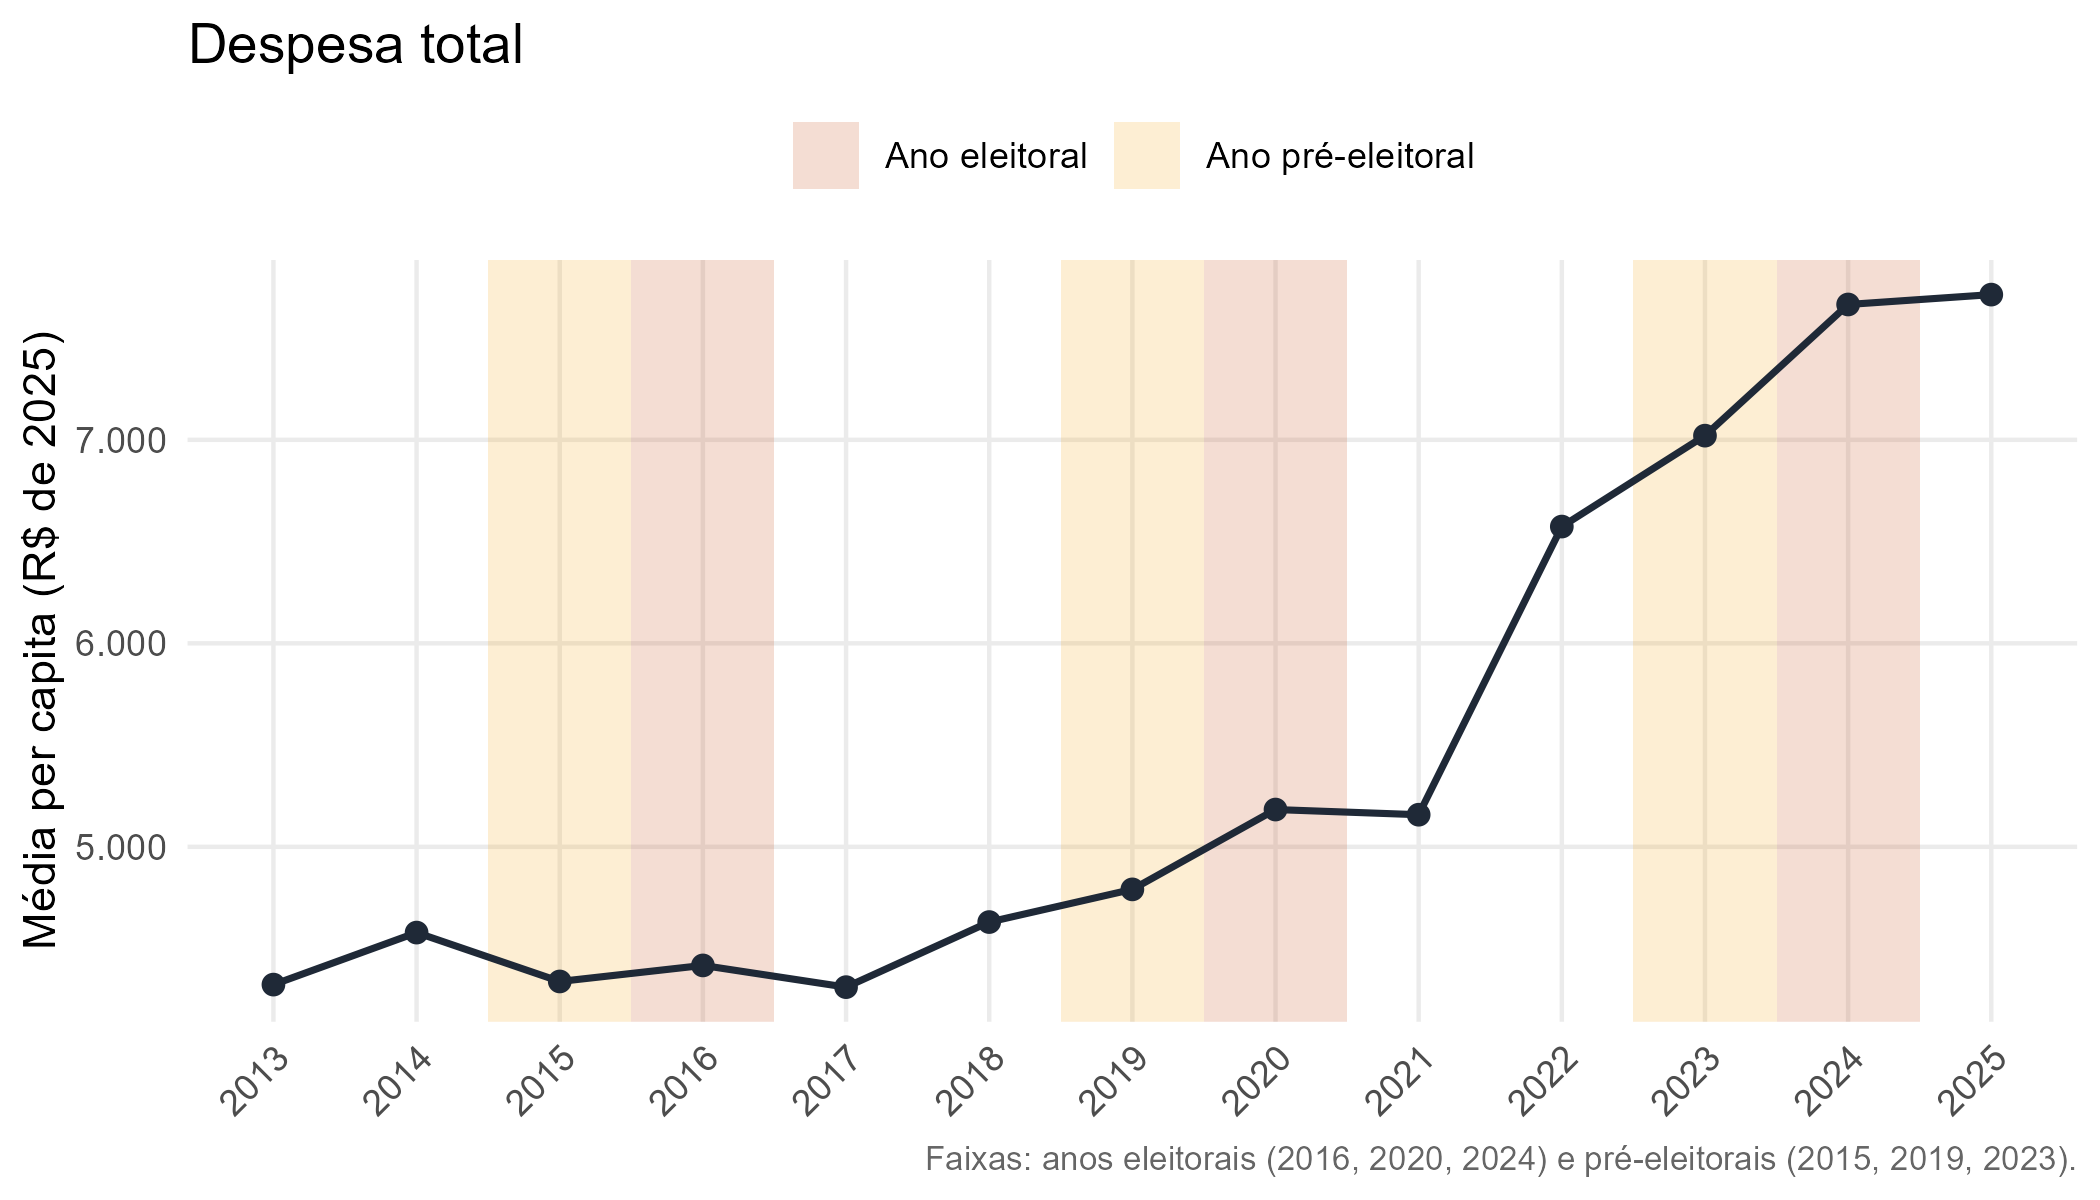
\includegraphics[width=0.9\textwidth]{fig/metodologia/serie_despesa_total_nivel.png}
\fonte{Elaboração própria com dados do Siconfi e do IBGE.}
\nota{Média simples, entre os municípios que informaram a despesa no ano, do valor per capita em reais de 2025. Faixas em laranja: anos eleitorais (2016, 2020 e 2024); em amarelo: anos pré-eleitorais (2015, 2019 e 2023).}
\end{figure}

\begin{figure}[htbp]
\caption{Despesa per capita por grupo de funções, média do logaritmo}\label{fig:grupos}
\centering
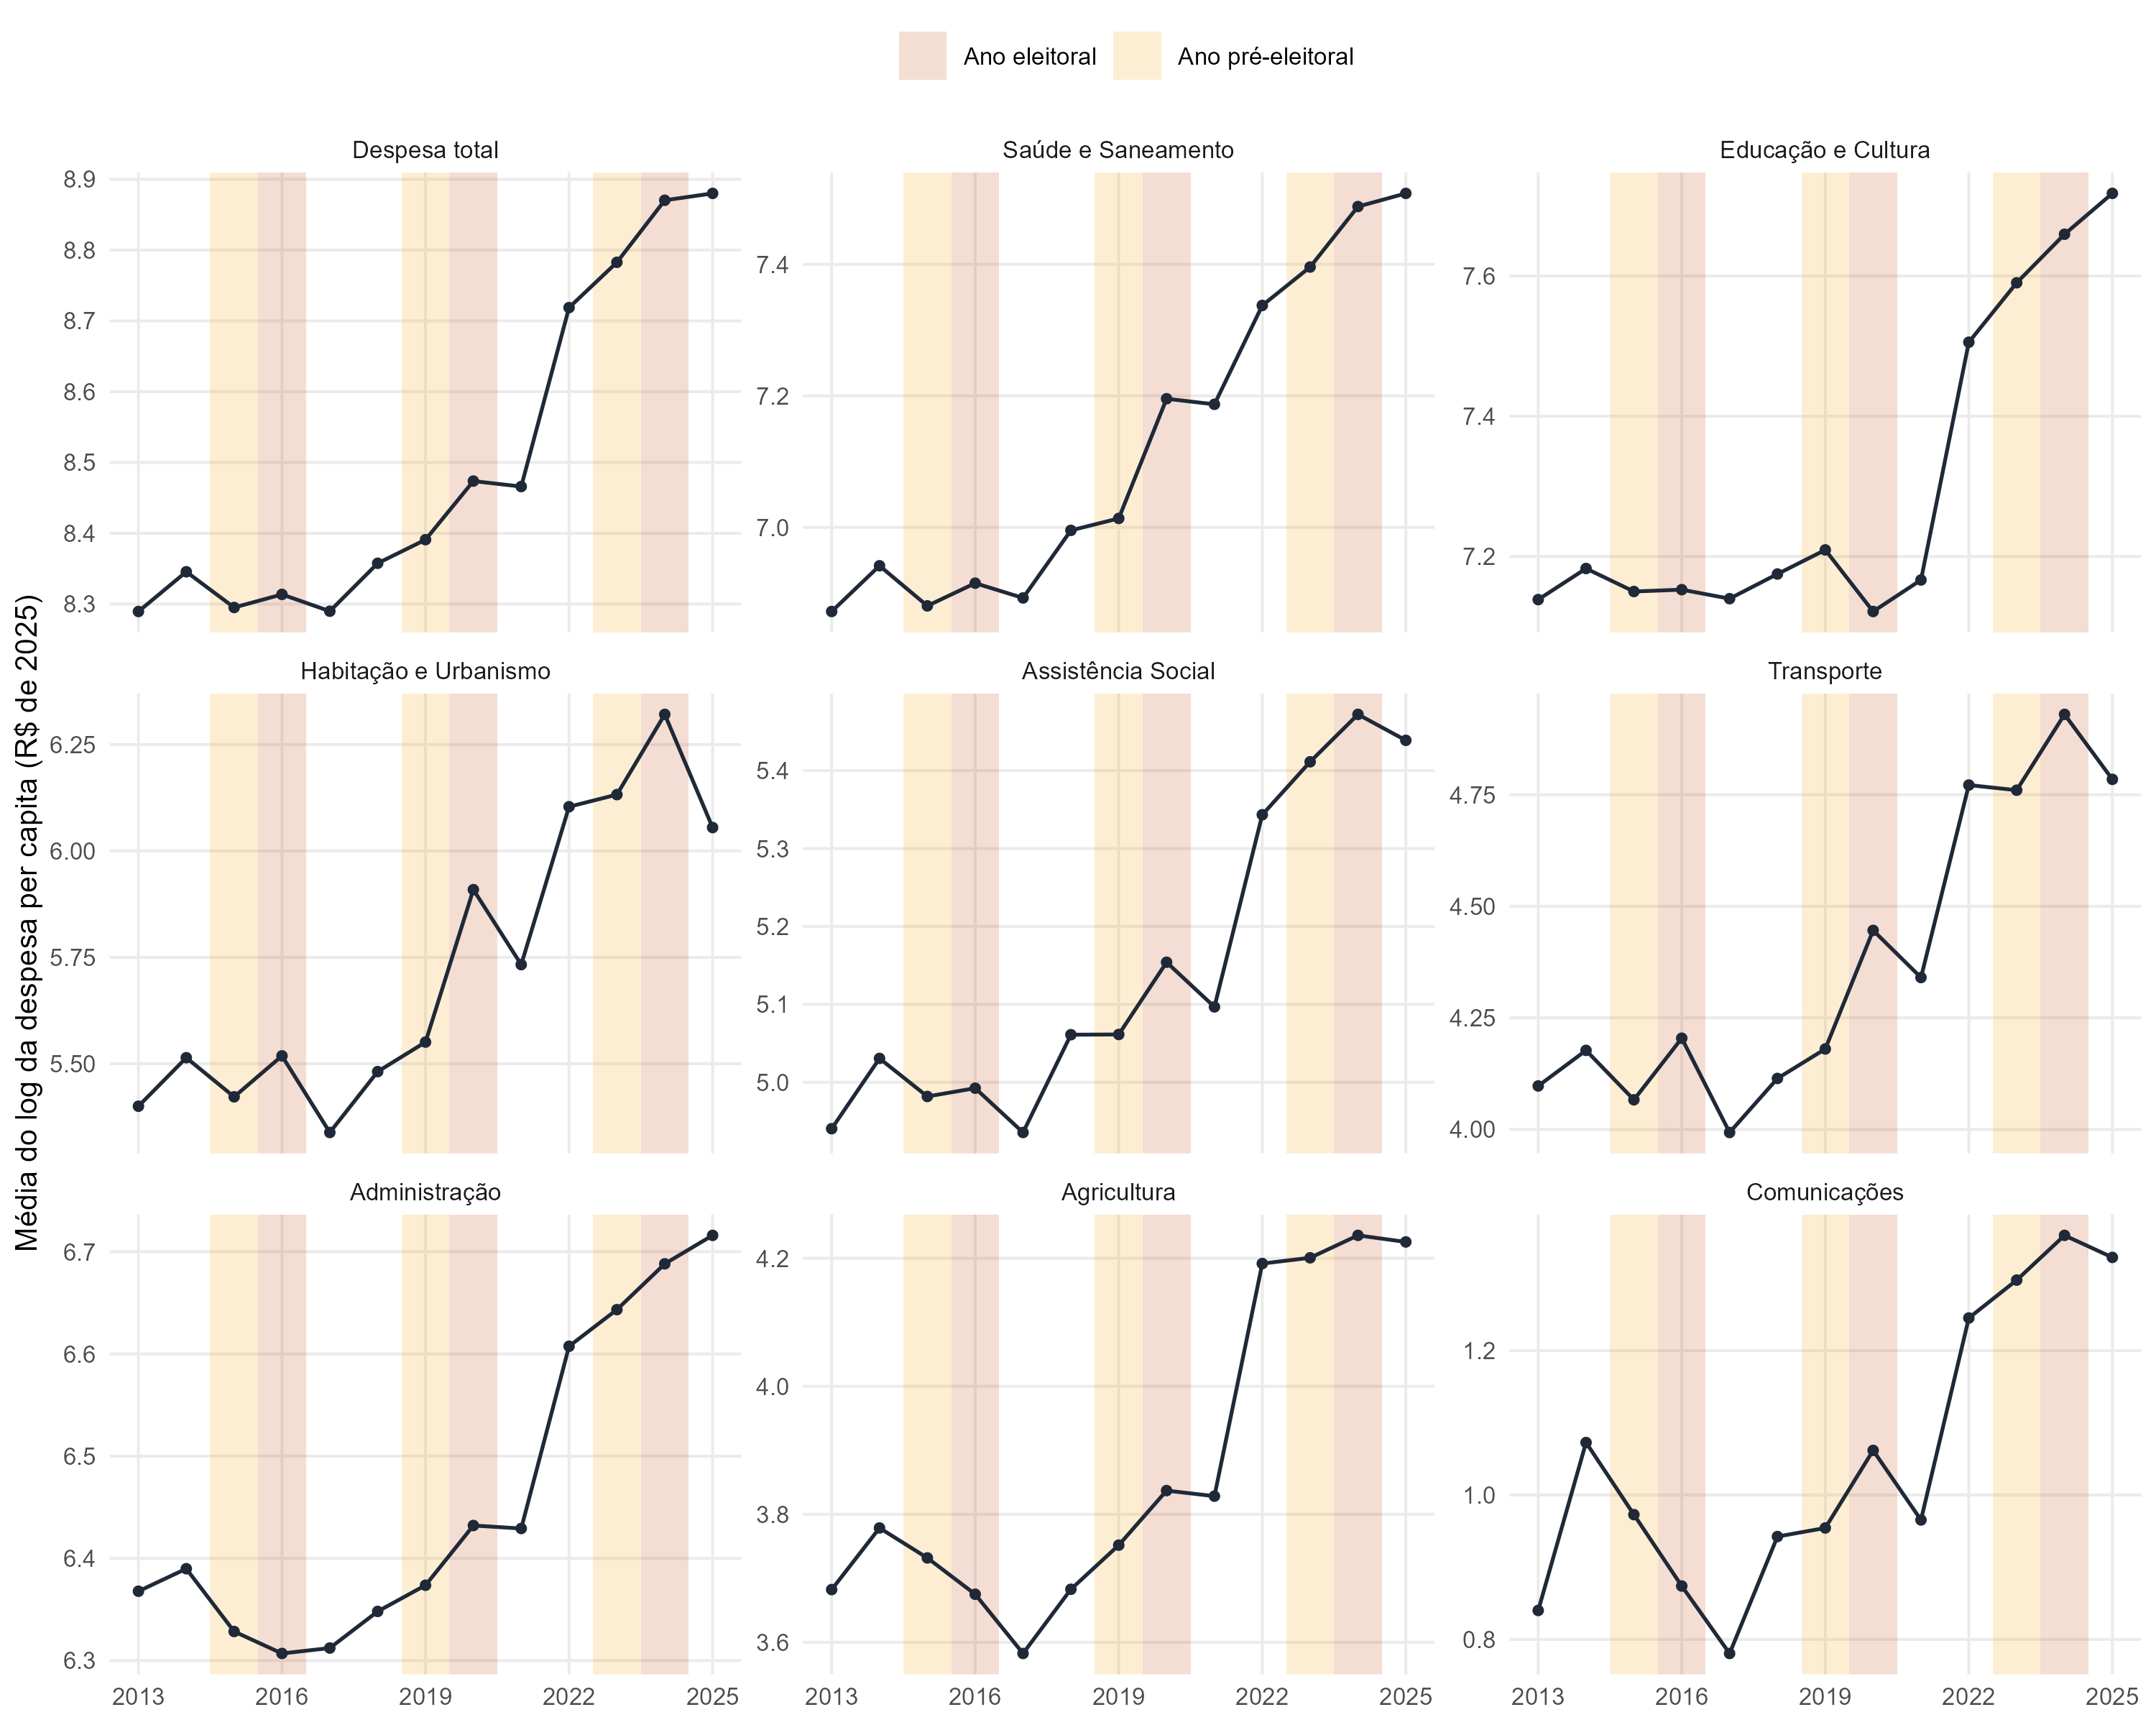
\includegraphics[width=\textwidth]{fig/metodologia/series_todas_log.png}
\fonte{Elaboração própria com dados do Siconfi e do IBGE.}
\nota{Média simples, entre os municípios que informaram a despesa no ano, do logaritmo da despesa per capita em reais de 2025. A escala logarítmica permite comparar variações relativas entre grupos de tamanhos diferentes. Faixas como na \autoref{fig:total}.}
\end{figure}

A despesa total per capita fica estável entre 2013 e 2017, entre R\$~4.300 e R\$~4.600, período que inclui a recessão de 2015--2016. Cresce de forma gradual entre 2018 e 2021 e salta de cerca de R\$~5.200 em 2021 para R\$~6.600 em 2022, chegando a quase R\$~7.700 em 2024 e 2025.

Habitação e Urbanismo e Transporte têm picos em 2016, 2020 e 2024 e quedas em 2017, 2021 e 2025. É o padrão previsto pela teoria dos ciclos políticos orçamentários: obras e serviços visíveis são concentrados no ano da eleição. Assistência Social também tem picos em 2020 e 2024.

Saúde e Saneamento sobe com força em 2020 e não volta ao nível anterior, o que mistura o efeito da pandemia com o da eleição daquele ano; esse é o motivo da dummy de pandemia no modelo. Educação e Cultura fica praticamente estável até 2021, cai em 2020 e salta em 2022, sem pico nos anos eleitorais, o que é coerente com a rigidez do gasto vinculado. Administração cai entre 2014 e 2016 e cresce depois, sem padrão eleitoral claro. Comunicações oscila muito, reflexo da amostra pequena.

A leitura gráfica sugere um ciclo eleitoral concentrado na composição do gasto, mas não separa a eleição de outros fatores do mesmo ano, como a pandemia em 2020 e o salto de 2022 em diante. A análise econométrica faz essa separação controlando receitas, demografia, PIB e tendência.

% ------------------------------------------------------------------------------
\section{Dados em painel}\label{sec:painel}

\subsection{O problema da variável omitida}

Dados em painel acompanham as mesmas unidades de corte transversal, aqui os municípios, ao longo de vários períodos. A principal vantagem sobre um único corte transversal é permitir controlar características não observadas que não mudam no tempo \parencite[p.~247--248]{wooldridge2002}. Se essas características forem correlacionadas com as variáveis explicativas e ficarem no termo de erro, o estimador de mínimos quadrados ordinários é viesado e inconsistente; com observações repetidas da mesma unidade, é possível eliminá-las.

No caso dos municípios, características como a cultura política local, a qualidade da gestão, a localização e a estrutura produtiva afetam o gasto e provavelmente se relacionam com o alinhamento político do prefeito e com as receitas. A amostra tem $N = 5.568$ municípios e $T = 13$ anos. Como $N$ é muito maior que $T$, vale a análise assintótica com $N$ grande e $T$ fixo adotada por \textcite[p.~250--251]{wooldridge2002}. O painel é desbalanceado, porque nem todos os municípios têm dados em todos os anos.

\subsection{O modelo de efeitos não observados}

O modelo básico \parencite[p.~251]{wooldridge2002} é
\begin{equation}\label{eq:uem}
y_{it} = \mathbf{x}_{it}\boldsymbol{\beta} + c_i + u_{it}, \qquad t = 1, \dots, T,
\end{equation}
em que $y_{it}$ é a despesa per capita do município $i$ no ano $t$, $\mathbf{x}_{it}$ é o vetor de variáveis explicativas, $c_i$ é o efeito não observado (heterogeneidade do município, constante no tempo) e $u_{it}$ é o erro idiossincrático, que varia entre municípios e ao longo do tempo.

Os estimadores apresentados a seguir exigem exogeneidade estrita das explicativas, condicional ao efeito não observado \parencite[p.~253]{wooldridge2002}:
\begin{equation}\label{eq:exog}
E(u_{it} \mid \mathbf{x}_{i1}, \dots, \mathbf{x}_{iT}, c_i) = 0, \qquad t = 1, \dots, T.
\end{equation}
Isto é: controlados $\mathbf{x}_{it}$ e $c_i$, as explicativas de outros anos não afetam a despesa do ano $t$. Para \textcite[p.~251--252]{wooldridge2002}, a diferença entre ``efeitos fixos'' e ``efeitos aleatórios'' não está em tratar $c_i$ como parâmetro ou como variável aleatória, e sim em saber se $c_i$ é correlacionado com as explicativas.

\subsection{Mínimos quadrados agrupados}

O estimador de mínimos quadrados agrupados (\textit{pooled}) trata a base como um único corte transversal, com erro composto $v_{it} = c_i + u_{it}$. Ele só é consistente se $c_i$ não for correlacionado com $\mathbf{x}_{it}$; mesmo assim, os erros de um mesmo município são correlacionados ao longo do tempo por causa de $c_i$, o que exige erros-padrão robustos \parencite[p.~256--257]{wooldridge2002}.

\subsection{Efeitos aleatórios}

O estimador de efeitos aleatórios mantém $c_i$ no erro e supõe que ele não tem relação com as explicativas de nenhum período \parencite[p.~257]{wooldridge2002}:
\begin{equation}\label{eq:re}
E(c_i \mid \mathbf{x}_{i1}, \dots, \mathbf{x}_{iT}) = E(c_i) = 0.
\end{equation}
Como $c_i$ aparece em todos os períodos, os erros compostos de um mesmo município são correlacionados. O estimador de efeitos aleatórios usa mínimos quadrados generalizados factíveis para aproveitar essa estrutura, o que equivale a aplicar mínimos quadrados agrupados aos dados ``quase centrados'' na média do município \parencite[p.~286--287]{wooldridge2002}:
\begin{equation}\label{eq:quasi}
y_{it} - \lambda \bar{y}_i = (\mathbf{x}_{it} - \lambda \bar{\mathbf{x}}_i)\boldsymbol{\beta} + (v_{it} - \lambda \bar{v}_i), \qquad
\lambda = 1 - \left[ \frac{\sigma_u^2}{\sigma_u^2 + T\sigma_c^2} \right]^{1/2},
\end{equation}
em que $\sigma_c^2$ e $\sigma_u^2$ são as variâncias do efeito não observado e do erro idiossincrático. Se a hipótese da \autoref{eq:re} vale, o estimador é consistente e mais eficiente que o de efeitos fixos, e permite estimar o efeito de variáveis constantes no tempo; se ela falha, ele é inconsistente. Neste trabalho, as variâncias foram estimadas pelo método de \textcite{wallace1969}, porque o método usual não pôde ser calculado na presença de variáveis que só variam no tempo (ano eleitoral, tendências e PIB nacional).

\subsection{Efeitos fixos}

O estimador de efeitos fixos permite que $c_i$ seja correlacionado de forma arbitrária com as explicativas: mantém apenas a exogeneidade estrita da \autoref{eq:exog} \parencite[p.~265--266]{wooldridge2002}. Para eliminar $c_i$, subtrai-se de cada variável a sua média no tempo dentro do município, a chamada transformação \textit{within} \parencite[p.~267]{wooldridge2002}:
\begin{equation}\label{eq:within}
y_{it} - \bar{y}_i = (\mathbf{x}_{it} - \bar{\mathbf{x}}_i)\boldsymbol{\beta} + (u_{it} - \bar{u}_i).
\end{equation}
Como $c_i$ é igual em todos os anos, ele desaparece, e $\boldsymbol{\beta}$ é estimado por mínimos quadrados agrupados na equação transformada. O resultado é idêntico ao de incluir uma variável dummy para cada município \parencite[p.~272]{wooldridge2002}. Intuitivamente, cada município é comparado consigo mesmo ao longo do tempo. O custo é que variáveis constantes no tempo não podem ser estimadas, e variáveis que variam pouco dentro do município são estimadas com pouca precisão \parencite[p.~266, 286]{wooldridge2002}.

Os dois estimadores estão ligados pelo parâmetro $\lambda$ da \autoref{eq:quasi}: com $\lambda = 0$, o de efeitos aleatórios coincide com o de mínimos quadrados agrupados; com $\lambda$ próximo de 1, aproxima-se do de efeitos fixos \parencite[p.~287]{wooldridge2002}.

\subsection{Teste de Hausman}

Como a escolha depende de $c_i$ ser ou não correlacionado com as explicativas, \textcite{hausman1978} propôs comparar as duas estimativas. Sob a hipótese nula, ambos os estimadores são consistentes e o de efeitos aleatórios é eficiente; sob a alternativa, só o de efeitos fixos é consistente. Uma diferença estatisticamente significativa é evidência contra os efeitos aleatórios \parencite[p.~288--289]{wooldridge2002}:
\begin{equation}\label{eq:hausman}
H = (\hat{\boldsymbol{\delta}}_{EF} - \hat{\boldsymbol{\delta}}_{EA})' \left[ \widehat{\mathrm{Avar}}(\hat{\boldsymbol{\delta}}_{EF}) - \widehat{\mathrm{Avar}}(\hat{\boldsymbol{\delta}}_{EA}) \right]^{-1} (\hat{\boldsymbol{\delta}}_{EF} - \hat{\boldsymbol{\delta}}_{EA}) \sim \chi^2_M,
\end{equation}
em que $\boldsymbol{\delta}$ reúne os coeficientes das $M$ variáveis que variam entre municípios e no tempo. A versão clássica supõe erros homocedásticos e sem correlação serial. Quando isso não vale, \textcite[p.~291]{wooldridge2002} recomenda uma versão robusta baseada em regressão, equivalente à de \textcite{mundlak1978}: acrescentam-se ao modelo as médias por município das explicativas e testa-se, com erros-padrão robustos, se seus coeficientes são conjuntamente nulos. Este trabalho reporta as duas versões.

\subsection{Erros-padrão}

Mesmo com efeitos fixos, os erros idiossincráticos podem ser heterocedásticos e correlacionados ao longo do tempo dentro do município. Por isso \textcite[p.~274--276]{wooldridge2002} recomenda uma matriz de variância robusta a heterocedasticidade e a correlação serial, que corresponde ao erro-padrão agrupado por município. Essa matriz, porém, supõe que municípios diferentes são independentes \parencite[p.~250]{wooldridge2002}. Para variáveis comuns a todos os municípios no mesmo ano, como o ano eleitoral, choques nacionais tornam os erros correlacionados entre municípios. Nesse caso usa-se o estimador de \textcite{driscoll1998}, robusto também à dependência entre municípios no mesmo período.

% ------------------------------------------------------------------------------
\section{Especificação empírica}\label{sec:especificacao}

São estimados dois modelos de efeitos fixos para cada uma das nove variáveis dependentes: o modelo A mede o ciclo eleitoral e o modelo B mede o efeito do alinhamento político.

\subsection{Escolha do estimador}

Em todas as nove variáveis, o teste de Hausman rejeita a hipótese nula, tanto na versão clássica quanto na robusta (\autoref{tab:hausman}). A heterogeneidade não observada dos municípios é, portanto, correlacionada com as explicativas, e o estimador de efeitos fixos é o adequado, como em \textcite{sakurai2009}.

\begin{table}[htbp]
\caption{Teste de Hausman: efeitos fixos contra efeitos aleatórios}\label{tab:hausman}
\centering
\footnotesize
\setlength{\tabcolsep}{4pt}
\begin{tabular}{lrrrr}
\hline
\textbf{Variável dependente} & \textbf{Clássico ($\chi^2$)} & \textbf{Robusto ($\chi^2$)} & \textbf{Observações} & \textbf{Municípios} \\ \hline
Despesa total & 3.573,83 & 267,50 & 70.669 & 5.568 \\
Saúde e Saneamento & 2.258,51 & 387,08 & 70.526 & 5.568 \\
Educação e Cultura & 3.911,60 & 1.113,39 & 70.550 & 5.568 \\
Habitação e Urbanismo & 179,95 & 42,92 & 69.574 & 5.564 \\
Assistência Social & 2.632,55 & 142,51 & 70.485 & 5.568 \\
Transporte & 944,72 & 273,29 & 54.423 & 5.205 \\
Administração & 1.627,32 & 121,72 & 70.553 & 5.568 \\
Agricultura & 857,00 & 264,36 & 64.464 & 5.436 \\
Comunicações & 154,56 & 35,63 & 12.360 & 1.896 \\ \hline
\end{tabular}
\fonte{Elaboração própria.}
\nota{Especificação do modelo A. Em todos os casos, p-valor $<$ 0,001 nas duas versões; hipótese nula: o estimador de efeitos aleatórios é consistente. Versão robusta: teste de \textcite{mundlak1978} com erros-padrão agrupados por município.}
\end{table}

\subsection{Modelo A: ciclo eleitoral}

Para o município $i$, o ano $t$ e o grupo de despesa $k$:
\begin{equation}\label{eq:modeloA}
\begin{split}
d^k_{it} = {} & \beta_1 \mathit{Eleitoral}_t + \beta_2 \mathit{PreEleitoral}_t + \beta_3 \mathit{Pandemia}_t + \gamma_1 \mathit{CoalGov}_{it} + \gamma_2 \mathit{CoalPres}_{it} \\
& + \mathbf{X}_{it}\boldsymbol{\delta} + \phi\, \mathit{PIB}_t + \theta_1 t + \theta_2 t^2 + c_i + u_{it},
\end{split}
\end{equation}
em que $d$ é a despesa per capita, $\mathbf{X}$ reúne os controles que variam entre municípios (receitas per capita, demografia, urbanização e logaritmo da população) e $c_i$ é o efeito fixo do município. Não se inclui efeito fixo de ano, porque as dummies eleitorais são iguais para todos os municípios no mesmo ano e seriam absorvidas por ele; o tempo é controlado pelo PIB nacional e pelas tendências linear e quadrática, como em \textcite{sakurai2009}. Os erros-padrão são de \textcite{driscoll1998}, porque o ano eleitoral é comum a todos os municípios e choques nacionais afetam todos ao mesmo tempo.

A dummy de pandemia vale 1 em 2020, que também é ano eleitoral. Com ela, o coeficiente $\beta_1$ é identificado pelas eleições de 2016 e 2024, e $\beta_3$ mede quanto 2020 se afastou de um ano eleitoral típico.

\subsection{Modelo B: coalizões}

\begin{equation}\label{eq:modeloB}
d^k_{it} = \gamma_1 \mathit{CoalGov}_{it} + \gamma_2 \mathit{CoalPres}_{it} + \mathbf{X}_{it}\boldsymbol{\delta} + c_i + \tau_t + u_{it},
\end{equation}
em que $\tau_t$ é o efeito fixo de ano. Ele absorve tudo o que atinge todos os municípios no mesmo ano: o calendário eleitoral, a pandemia, o ciclo econômico e mudanças de regras nacionais. Assim, o alinhamento é medido comparando, dentro do mesmo ano, prefeitos alinhados e não alinhados. Isso é necessário porque a proporção de prefeitos na coalizão do presidente muda com cada governo federal (\autoref{tab:politicas}); sem o efeito de ano, o coeficiente misturaria o alinhamento com o período. Os erros-padrão são agrupados por município \parencite[p.~274--276]{wooldridge2002}.

\subsection{Interpretação dos coeficientes}

Os coeficientes estão em reais de 2025 per capita: $\beta_1 = 50$, por exemplo, indica que no ano eleitoral o município gasta R\$~50 a mais por habitante naquele grupo, mantidos os demais fatores. Um resultado é considerado sólido quando é significativo tanto com o erro de \textcite{driscoll1998} quanto com o erro agrupado por município, porque o estimador de Driscoll e Kraay perde precisão quando há poucos períodos, como aqui (13 anos).

% ------------------------------------------------------------------------------
\section{Testes de robustez}\label{sec:robustez}

Cada teste reestima os modelos mudando uma decisão da especificação principal. Quatro testes são discutidos no texto, por tratarem das decisões que mais podem afetar as conclusões:

\begin{enumerate}
\item \textbf{Especificação de \textcite{sakurai2009}}: modelo A sem ano pré-eleitoral e sem dummy de pandemia, com erro agrupado por município, para comparar com a literatura;
\item \textbf{Erro-padrão agrupado por município} no modelo A, em vez de Driscoll e Kraay, para verificar se a significância depende do tipo de erro;
\item \textbf{Modelo A sem a dummy de pandemia}, em que 2020 volta a contar como ano eleitoral comum e o efeito eleitoral é medido pelas três eleições;
\item \textbf{Um efeito para cada eleição}: o ano eleitoral é dividido em dummies para 2016 e para 2024, e o pré-eleitoral em dummies para 2015, 2019 e 2023, para verificar se o efeito médio vem de uma única eleição.
\end{enumerate}

Os demais testes, que tratam da regra de padronização das siglas, das eleições suplementares, da forma funcional, da limpeza da base, do registro irregular de algumas funções e dos controles, estão descritos no \autoref{ap:robustez}.
